\chapter{PHÂN TÍCH LỖI VÀ THẢO LUẬN}
\label{chap:a-discussion}

\section{Triage lỗi theo bước pipeline}
\label{sec:triage}

Để biết pipeline mất ảnh ở đâu, mỗi ảnh test được gán đúng một \emph{bước lỗi chính}, xét theo thứ tự pipeline. Cấu hình: định vị \code{edge\_svm} + bilateral, crop quad, nhị phân Otsu, tách ký tự CCA (như E4). Bảng~\ref{tab:stagedef} định nghĩa các bước; kết quả đếm ở Bảng~\ref{tab:triage} và Hình~\ref{fig:triage}.

\begin{table}[htbp]
\centering
\caption{Định nghĩa bước lỗi chính (ưu tiên từ trên xuống).}
\label{tab:stagedef}
\small
\rowcolors{2}{white}{tablerowalt}
\arrayrulecolor{tableheader}
\begin{tabularx}{\textwidth}{lY}
\hline
\rowcolor{tableheader} \tblhd{Bước} & \tblhd{Điều kiện} \\
\hline
\code{loc\_no\_candidate} & không ứng viên nào trong top-5 có IoU $\ge 0.5$ với bbox thật \\
\code{loc\_rank} & có ứng viên đúng trong top-5 nhưng không phải top-1 \\
\code{rectify} & top-1 đúng, không \code{all\_correct}, và sai số góc quad lớn hơn ngưỡng \\
\code{segment\_count} & top-1 đúng, nắn ổn, nhưng số hộp ký tự khác 7 \\
\code{segment\_position} & đủ 7 hộp nhưng có vị trí không trúng khuôn \\
\code{ok} & top-1 đúng và \code{all\_correct} \\
\hline
\end{tabularx}
\end{table}

Ngưỡng sai số góc là $22.30$ px, bằng phân vị 95 của sai số góc trên tune trong số ảnh top-1 đúng và tách đúng hết ($n=50$ trong 159 ảnh top-1 đúng; trung vị 10.84 px, trong khi nhóm top-1 đúng nhưng tách sai có trung vị 19.84 px). Nói cách khác, đó là mức sai số mà ảnh tách tốt còn chịu được. Ngưỡng tính bằng pixel của ảnh gốc nên phụ thuộc kích thước biển trong ảnh. Ngưỡng chọn trên tune, không dùng số test. Ảnh nắn lệch nhưng vẫn tách đúng thì là \code{ok}; ảnh top-1 sai không bao giờ là \code{ok}.

\begin{table}[htbp]
\centering
\caption[Số ảnh test theo bước lỗi chính và nhóm]{Số ảnh test theo bước lỗi chính và nhóm (trong ngoặc là số ảnh của nhóm); cột cuối là phần trăm trên toàn test ($n=462$). Nguồn: \code{triage\_stage\_counts.csv}.}
\label{tab:triage}
\footnotesize
\setlength{\tabcolsep}{3pt}
\rowcolors{2}{white}{tablerowalt}
\arrayrulecolor{tableheader}
\begin{tabularx}{\textwidth}{lCCCCCCC}
\hline
\rowcolor{tableheader} \tblhd{Bước} & \tblhd{base (350)} & \tblhd{blur (28)} & \tblhd{challenge (28)} & \tblhd{db (28)} & \tblhd{tilt (28)} & \tblhd{ALL (462)} & \tblhd{\% ALL} \\
\hline
loc\_no\_candidate & 44 & 10 & 14 & 16 & 12 & 96 & 20.8 \\
loc\_rank & 14 & 2 & 0 & 1 & 2 & 19 & 4.1 \\
rectify & 40 & 4 & 4 & 2 & 9 & 59 & 12.8 \\
segment\_count & 100 & 11 & 7 & 4 & 1 & 123 & 26.6 \\
segment\_position & 67 & 1 & 1 & 2 & 4 & 75 & 16.2 \\
ok & 85 & 0 & 2 & 3 & 0 & 90 & 19.5 \\
\hline
\end{tabularx}
\end{table}


Kiểm tra chéo với E3 và E6: \code{ok} $=90=0.1948\times 462$, khớp \code{all\_correct} của crop \code{pred} quad ở E4 và của tách \code{cca} với crop \code{pred} ở E6 (cả hai đều 0.1948); \code{loc\_no\_candidate} $+$ \code{loc\_rank} $=115=462-347$, khớp số ảnh top-1 sai của \code{edge\_svm}.

\begin{figure}[htbp]
\centering
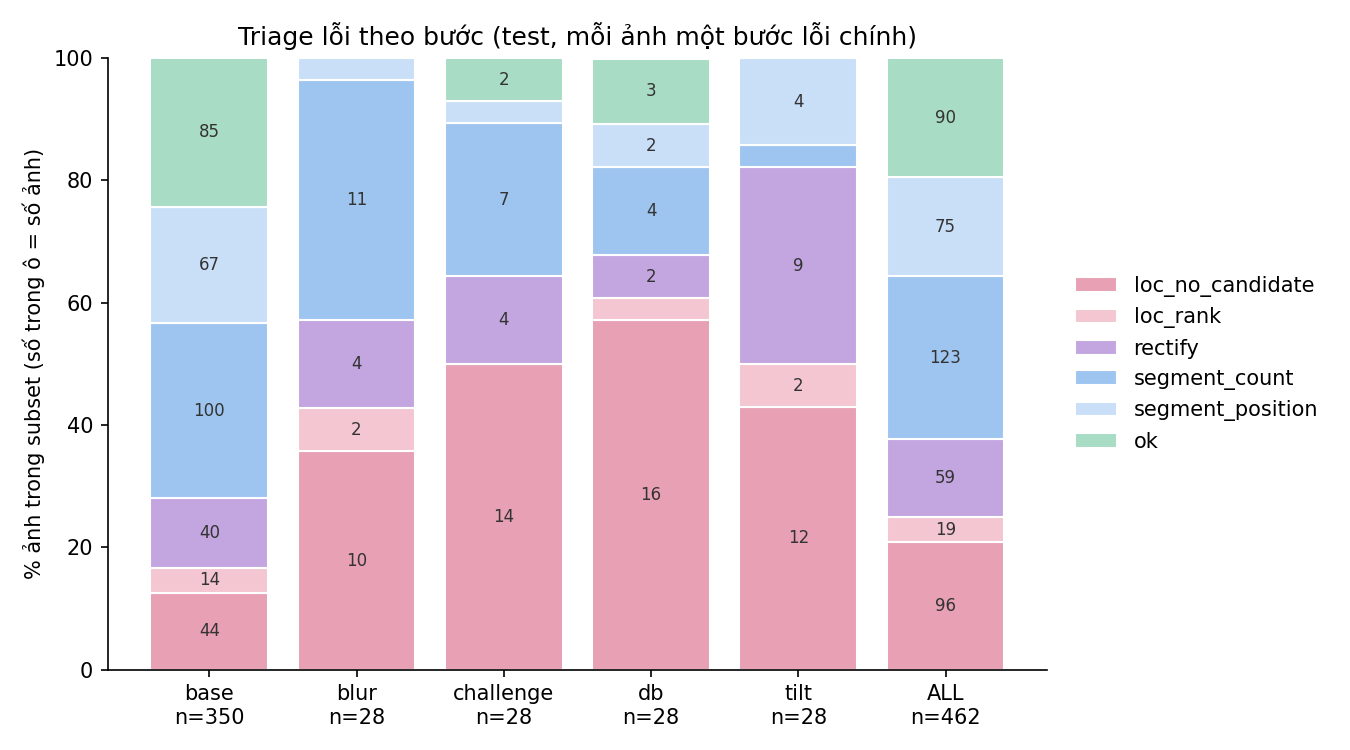
\includegraphics[width=0.85\textwidth]{figures/triage_stages.png}
\caption[Phân bố bước lỗi chính theo nhóm (test)]{Phân bố bước lỗi chính theo nhóm (test); số trong ô là số ảnh. Nguồn: \code{triage\_stage\_counts.csv}.}
\label{fig:triage}
\end{figure}

\textbf{Đọc bảng.} Theo Bảng~\ref{tab:triage} (và Hình~\ref{fig:triage}), chỉ 19.5\% ảnh test đi hết pipeline đúng. Lỗi lớn nhất là tách ký tự (\code{segment\_count} 26.6\% và \code{segment\_position} 16.2\%, tổng 42.8\%), kế đến là định vị (\code{loc\_no\_candidate} 20.8\% và \code{loc\_rank} 4.1\%, tổng 24.9\%) và nắn (12.8\%). Hai kiểu lỗi định vị rất khác nhau: \code{loc\_rank} (19 ảnh) là lỗi xếp hạng, \code{loc\_no\_candidate} (96 ảnh) là lỗi sinh ứng viên và lớn gấp năm lần. Trong 96 ảnh đó, 30 ảnh không có ứng viên nào và 66 ảnh có ứng viên nhưng đều IoU $<0.5$; chỉ 12 ảnh có bbox thật nhỏ hơn cận dưới \code{area\_ratio} (3 \code{base}, 1 \code{blur}, 7 \code{challenge}, 1 \code{db}), còn 84 ảnh thuộc nhóm ``khác'', nghĩa là bộ lọc diện tích chỉ giải thích được một phần nhỏ. Các nhóm khó gần như không có ảnh \code{ok} (0--3 trên 28 ảnh) và mất chủ yếu ở định vị (\code{loc\_no\_candidate} từ 36\% đến 57\%) và nắn (riêng \code{tilt}: 9/28 ảnh \code{rectify}), trừ \code{blur}: ở nhóm này định vị (12 ảnh) và tách ký tự (12 ảnh) mất bằng nhau. Nhóm \code{base} mất nhiều nhất ở tách ký tự (167/350 ảnh).

\textbf{Bảng chéo crop \code{gt} và crop \code{pred}.} Để phân biệt lỗi do định vị/nắn với lỗi do bộ tách ký tự, Bảng~\ref{tab:cross} đếm số ảnh theo trạng thái tách khi crop từ bbox/quad thật (hàng) và bước lỗi khi crop từ dự đoán (cột).

\begin{tabular}{lrrrrrr}
\toprule
crop gt $\backslash$ bước pred & loc\_no\_candidate & loc\_rank & rectify & segment\_count & segment\_position & ok \\
\midrule
ok (260) & 34 & 8 & 32 & 64 & 56 & 66 \\
segment\_count (182) & 57 & 8 & 21 & 57 & 15 & 24 \\
segment\_position (20) & 5 & 3 & 6 & 2 & 4 & 0 \\
\bottomrule
\end{tabular}


Trong 257 ảnh top-1 đúng nhưng vẫn lỗi (\code{rectify} $+$ \code{segment}), 152 ảnh tách đúng khi crop \code{gt}, tức lỗi do crop dự đoán (nắn lệch hoặc bbox không khít); 105 ảnh tách sai ngay cả với crop \code{gt}, tức lỗi do bộ tách. Hai nguồn này cùng bậc, nên cải thiện định vị/nắn và cải thiện bộ tách ký tự đều cần thiết. Còn 42 ảnh tách đúng ở crop \code{gt} nhưng hỏng ở định vị (34 \code{loc\_no\_candidate}, 8 \code{loc\_rank}) là lỗi thuần của định vị. Có 24 ảnh (trong 202 ảnh crop \code{gt} lỗi, khoảng 12\%) crop \code{gt} tách sai nhưng crop \code{pred} lại \code{ok}: viền cắt khác nên ký tự không dính, tức crop dự đoán tình cờ tốt hơn crop thật; tỉ lệ này không nhỏ.

\section{Quan sát định tính}
\label{sec:qual}

Hình~\ref{fig:grids} cho một ví dụ cho mỗi bước lỗi, trích từ các lưới gỡ lỗi (ứng viên đỏ và bbox thật xanh, mặt nạ morph, crop dự đoán và crop \code{gt} cùng ảnh nhị phân và hộp ký tự). Mỗi bước chọn 12 ảnh theo seed 42 để đọc; dưới đây là các quan sát từ lưới đó và từ bảng đếm.

\begin{figure}[htbp]
\centering
\begin{subfigure}[t]{0.48\textwidth}
  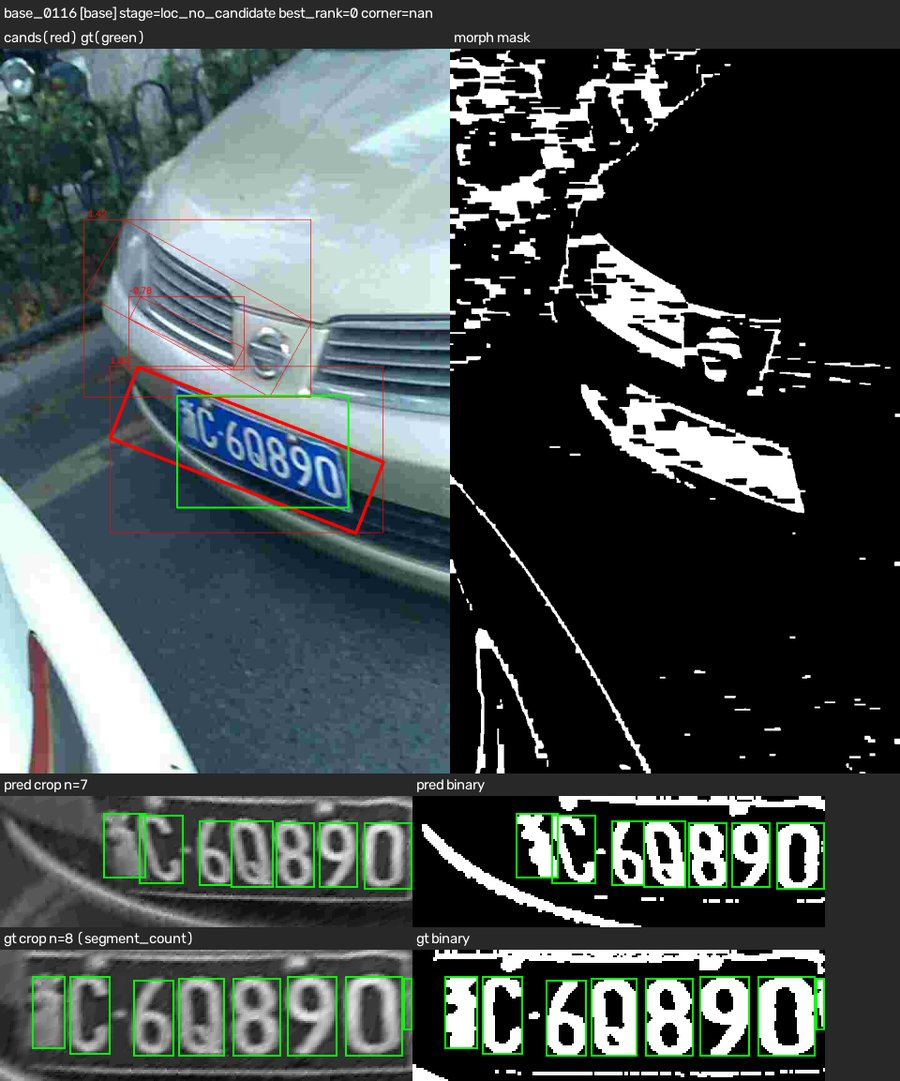
\includegraphics[width=\textwidth,height=0.255\textheight,keepaspectratio]{figures/grid_loc_no_candidate.jpg}
  \caption{\code{loc\_no\_candidate}}
\end{subfigure}\hfill
\begin{subfigure}[t]{0.48\textwidth}
  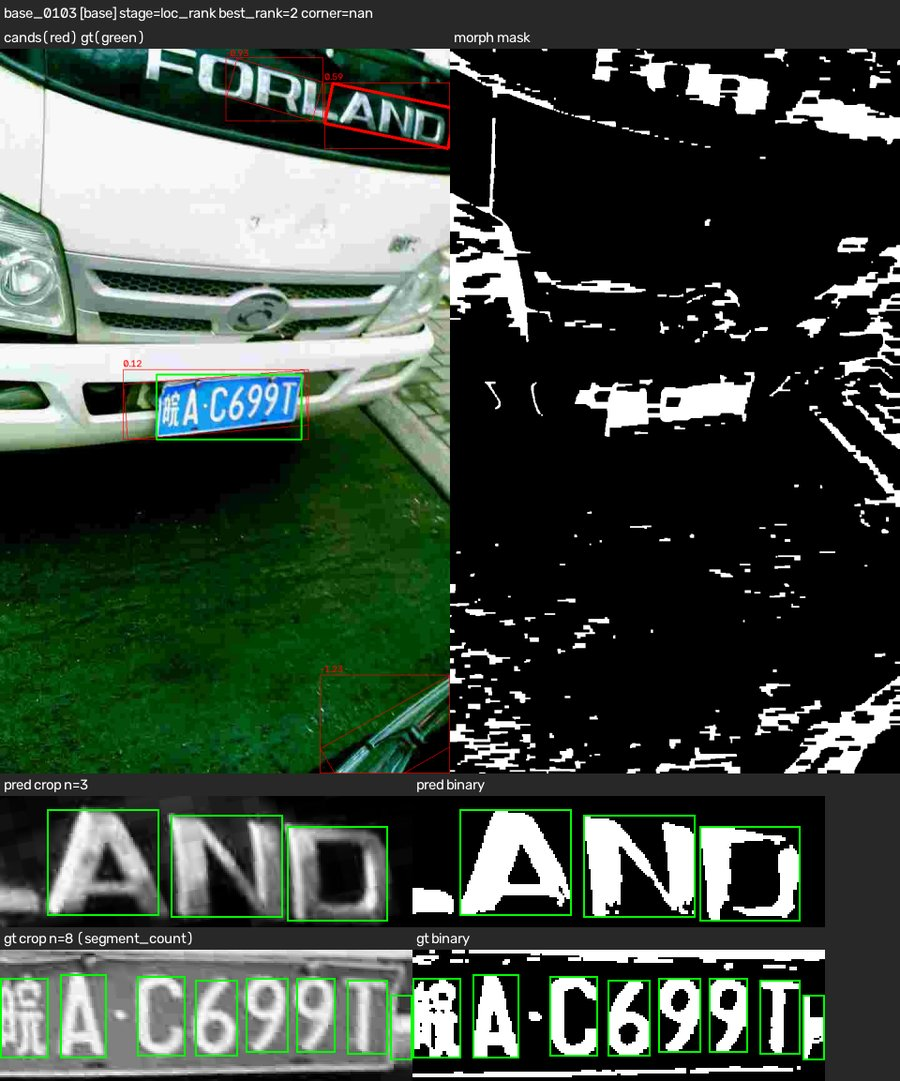
\includegraphics[width=\textwidth,height=0.255\textheight,keepaspectratio]{figures/grid_loc_rank.jpg}
  \caption{\code{loc\_rank}}
\end{subfigure}

\medskip
\begin{subfigure}[t]{0.48\textwidth}
  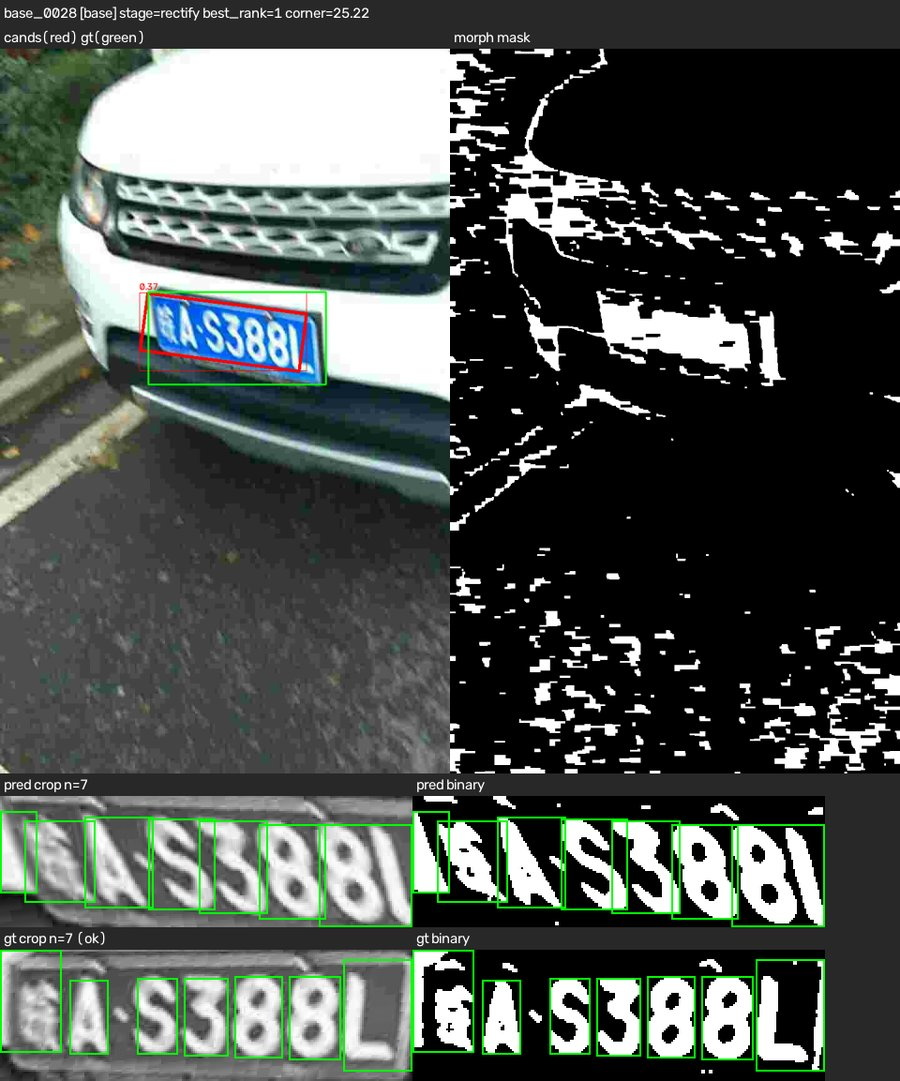
\includegraphics[width=\textwidth,height=0.255\textheight,keepaspectratio]{figures/grid_rectify.jpg}
  \caption{\code{rectify}}
\end{subfigure}\hfill
\begin{subfigure}[t]{0.48\textwidth}
  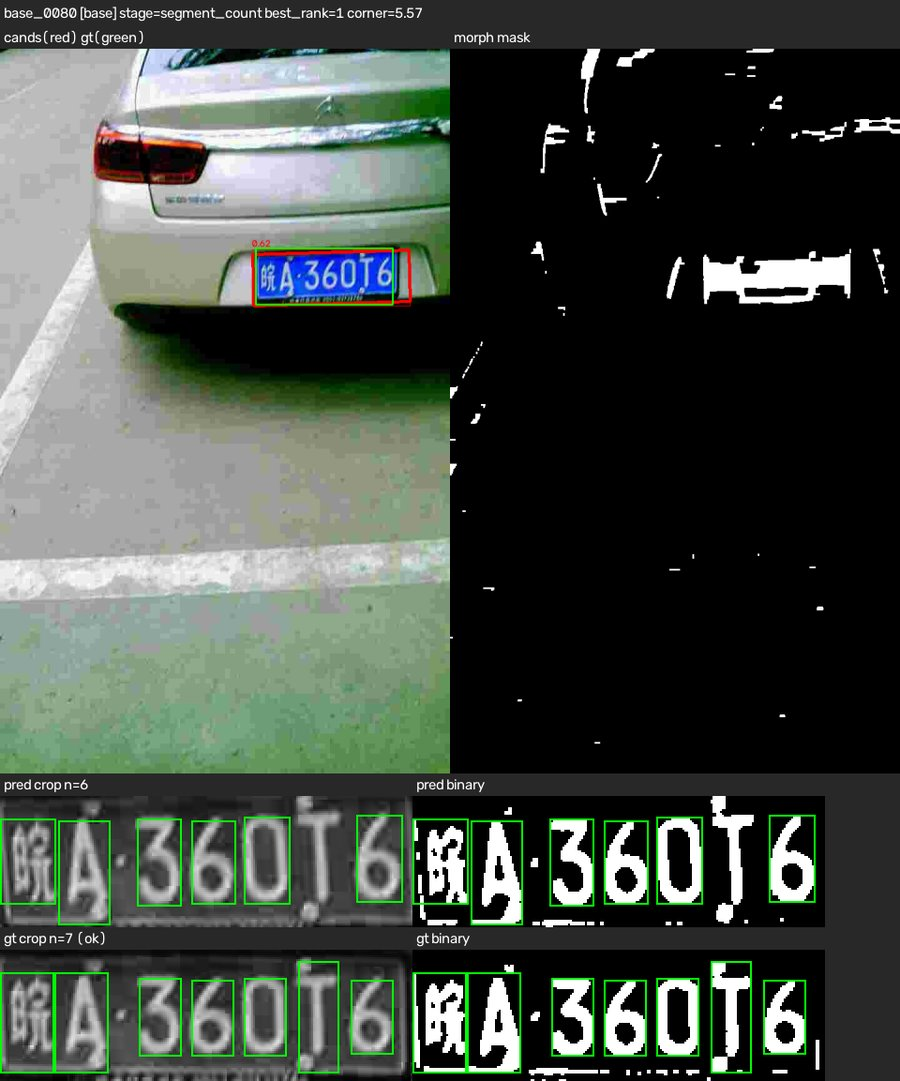
\includegraphics[width=\textwidth,height=0.255\textheight,keepaspectratio]{figures/grid_segment_count.jpg}
  \caption{\code{segment\_count}}
\end{subfigure}

\medskip
\begin{subfigure}[t]{0.48\textwidth}
  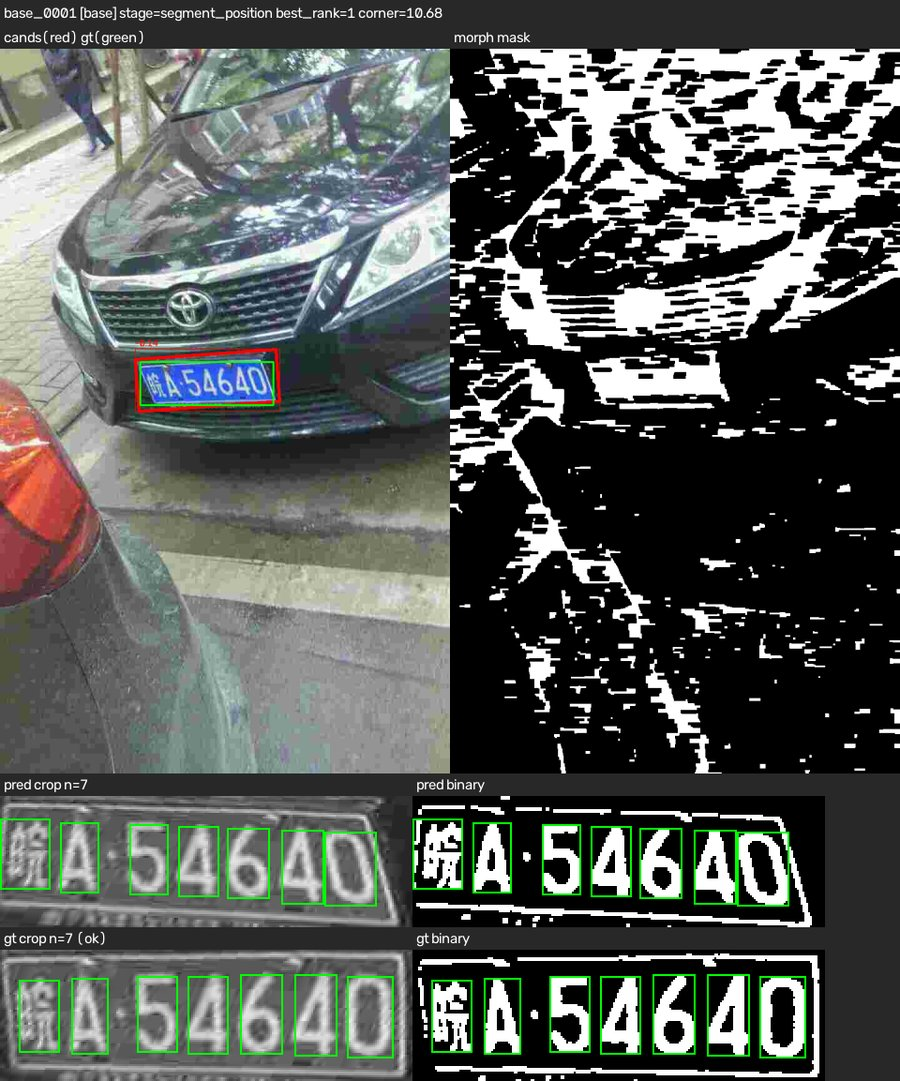
\includegraphics[width=\textwidth,height=0.255\textheight,keepaspectratio]{figures/grid_segment_position.jpg}
  \caption{\code{segment\_position}}
\end{subfigure}
\caption[Mỗi bước lỗi một ví dụ (test)]{Mỗi bước lỗi một ví dụ trên tập test (ảnh \code{base\_0116}, \code{base\_0103}, \code{base\_0028}, \code{base\_0080}, \code{base\_0001}). Hình gốc có độ phân giải cao hơn, có thể phóng to trong bản PDF.}
\label{fig:grids}
\end{figure}

\begin{itemize}
  \item \textbf{\code{loc\_no\_candidate}.} Ba dạng thường gặp: (1) ứng viên top-1 bao cả biển lẫn phần thân xe hoặc khung nên IoU thấp dù nhìn bằng mắt là trúng; biển nghiêng bị bbox ngang phạt nặng; (2) biển dính vào lưới tản nhiệt hoặc cản xe nên vùng sau morph không tách ra; (3) ảnh \code{challenge} nắng gắt, nhợt màu: mặt nạ morph phủ cả nền nhà và biển chỉ được điểm rất thấp (khoảng 0.01). Có 47/96 ảnh mà crop dự đoán không cho hộp ký tự nào.
  \item \textbf{\code{loc\_rank}.} 18 trong 19 ảnh có biển đúng ở hạng 2. Top-1 thường là chữ hãng xe hoặc logo ở đầu xe, có cạnh đứng dày (ví dụ chữ ``FORLAND'' trong Hình~\ref{fig:grids}b), mà SVM cho điểm cao hơn biển thật. Điều này gợi ý SVM chưa học đủ mẫu âm dạng chữ lớn trên nền tối.
  \item \textbf{\code{rectify}.} Warp thường cắt cụt hoặc làm lệch biển nên crop thiếu ký tự: trong 59 ảnh nhóm này, số hộp ký tự dự đoán là 0 (8 ảnh), 1 (4), 2 (1), 3 (1), 4 (5), 5 (13), 6 (9), 7 (13), 8 (4), 9 (1); chỉ 5/59 ảnh có 8--9 hộp và 41/59 có không quá 6 hộp (trung bình 4.75). Sai số góc trung bình của nhóm này là 34.9 px (so với 10.8 px của nhóm \code{ok}). Nhóm này nằm nhiều ở \code{tilt} (9/28) và \code{base}.
  \item \textbf{\code{segment\_count}.} Chủ yếu 6 hộp (54/123 ảnh) do ký tự Hán dính ký tự A (cả crop \code{gt} cũng bị), và 8 hộp (27/123) do mảnh nền hoặc khung biển ở mép; 64/123 ảnh này tách đúng trên crop \code{gt}.
  \item \textbf{\code{segment\_position}.} Đủ 7 hộp nhưng lệch khuôn vài pixel, thường ở ký tự Hán (nét rời, dính A), chữ số ``1'' hẹp và ký tự cuối chạm viền; crop dự đoán hơi lệch hoặc co làm cả dãy hộp trượt khỏi khuôn.
  \item {\sloppy \textbf{Theo mức nghiêng và mờ.} Mã hóa CCPD cho góc nghiêng ngang/dọc và độ mờ; chỉ dùng so sánh tương đối. Trung bình, ảnh \code{ok} có giá trị nghiêng cao nhất (86 và 82) so với \code{loc\_no\_candidate} (48 và 47) và \code{rectify} (66 và 63); độ mờ trung bình 58 ở \code{ok} so với 45 ở \code{loc\_no\_candidate}. Các giá trị này theo quy ước mã hóa của CCPD nên không nên hiểu là góc thật hay độ mờ thật.\par}
\end{itemize}

\section{Hạn chế}
\label{sec:limits}

\begin{itemize}
  \item \textbf{Cận diện tích của bộ lọc.} Trên test, 16/462 bbox thật nhỏ hơn cận dưới \code{area\_ratio} 0.008 (và 1 bbox lớn hơn 0.16). Đây không phải trần cứng: bộ lọc xét diện tích \code{minAreaRect} của ứng viên và IoU $\ge 0.5$ cho phép ứng viên lớn hơn bbox thật. Triage cho thấy chỉ 12/16 bbox nhỏ bị mất ở định vị (4 ảnh còn lại không mất ở đó), còn bbox lớn duy nhất (0.182) là lỗi xếp hạng \code{loc\_rank}.
  \item \textbf{IoU trục ngang phạt biển nghiêng.} Độ đo IoU dùng bbox ngang, nên biển nghiêng bị chấm thấp dù ứng viên bám đúng biển; điều này góp phần vào \code{loc\_no\_candidate}. Chưa dùng IoU của đa giác nghiêng.
  \item \textbf{Thời gian đo trên máy không rảnh.} Lần chạy dùng trong báo cáo (khoảng 140 ms/ảnh) đo trên máy ít tải hơn lần ghi trong sổ (416 ms/ảnh) nhưng vẫn không phải máy chuyên dụng. Tỉ lệ giữa các bước cũng dịch theo tải máy (tiền xử lý 44\% $\to$ 50\%, Sobel cùng morph 51\% $\to$ 45\%), nên chỉ xem là gần đúng; số đo lại ghi ở mục ``Đo lại thời gian (máy ít tải)'' trong \code{notes.md}.
  \item \textbf{Rò rỉ nhẹ ở kiểm chứng chéo của SVM.} Chia fold theo patch chứ không theo ảnh, nên số CV (F1 0.919) lạc quan; số định vị trên test mới phản ánh chất lượng thực. Số tune của \code{edge\_svm} cũng lạc quan vì huấn luyện trên chính tune.
  \item \textbf{Các nhóm khó rất nhỏ.} Mỗi nhóm \code{blur}, \code{db}, \code{challenge}, \code{tilt} chỉ 28 ảnh test (12 ảnh tune); một ảnh là 0.036, nên các so sánh (kể cả ngoại lệ \code{blur} ở E4) có độ bất định lớn. Chúng tôi chưa tính khoảng tin cậy và chỉ có một lần chia tune/test.
  \item \textbf{Một số lựa chọn dựa trên tune nhỏ.} Việc chọn \code{approxpoly} dựa trên 128 ảnh tune và khác biệt không có ý nghĩa thống kê; ngưỡng triage 22.3 px dựa trên 50 ảnh.
\end{itemize}

\section{Hướng cải thiện}

Vì 21\% ảnh test không có ứng viên đúng trong top-5, ưu tiên là bổ sung khâu sinh ứng viên, ví dụ thêm nguồn ứng viên theo màu biển hoặc bù nghiêng trước bước morph (chưa thử). Ở khâu xếp hạng, có thể thêm mẫu âm khó (chữ hãng xe, logo) vào SVM và chia fold theo ảnh khi kiểm chứng. Ở khâu nắn, cần quad chính xác hơn vì sai số khoảng 16 px nhiều khả năng góp phần đáng kể vào lỗi (giả thuyết; 152/257 ảnh top-1 đúng nhưng lỗi tách đúng khi crop \code{gt}); và dùng IoU đa giác để đánh giá công bằng hơn với biển nghiêng. Lỗi dính ký tự Hán với chữ A thuộc phần tách ký tự và được nêu ở phần của B.
